\section{Results and Discussion}

\subsection{Emulating System Dynamics}
Due to the continuous time-semantics which can be expressed in our ABS approach we can also emulate system dynamics. Every stock and flow is then just an agent which exchange messages where the simulation is stepped using the \textit{parallel} update-strategy. We add wrappers and type-definitions for convenience which increases the expressivity of the code, resembling system dynamics specifications. As a proof-of-concept we emulated the system dynamics of the SIR model, the code can be seen in Appendix \ref{app:sd_code}. Note that the code really looks like a system dynamics specification with the integrals of the mathematical specification directly showing up in the code - the implementation is correct per definition. Due to the internal implementation of the \textit{integral} function of Yampa which uses the rectangle-rule to integrate, one must ensure to sample the system dynamics with small enough $t\Delta$ as can be seen in Figure \ref{fig:sd_plots}.

\begin{figure*}
\begin{center}
	\begin{tabular}{c c}
		\begin{subfigure}[b]{0.5\textwidth}
			\centering
			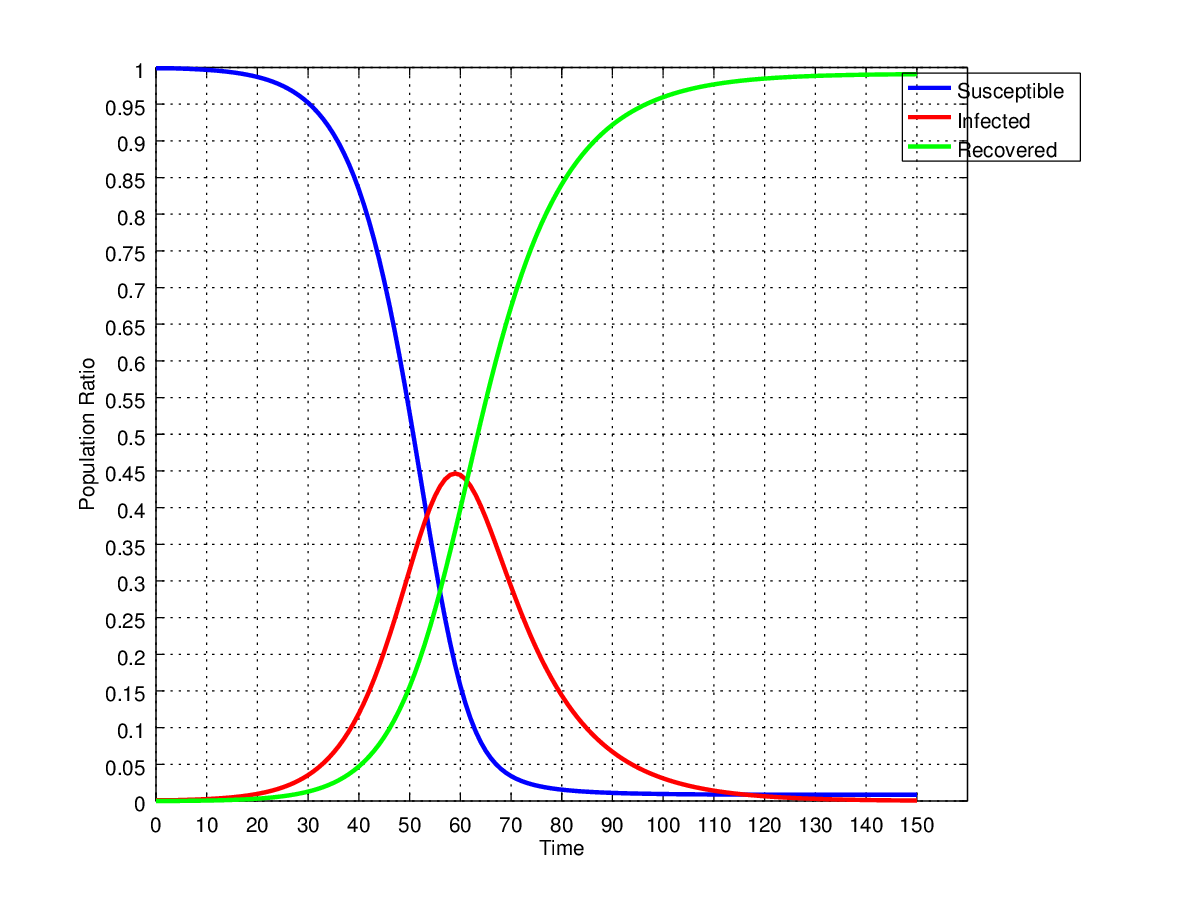
\includegraphics[width=.8\textwidth, angle=0]{./../shared/fig/frsd/SIR_SD_1000agents_150t_1dt.png}
			\caption{$t\Delta = 1.0$}
			\label{fig:sd_plot_10dt}
		\end{subfigure}
	
		& 
		
		\begin{subfigure}[b]{0.5\textwidth}
			\centering
			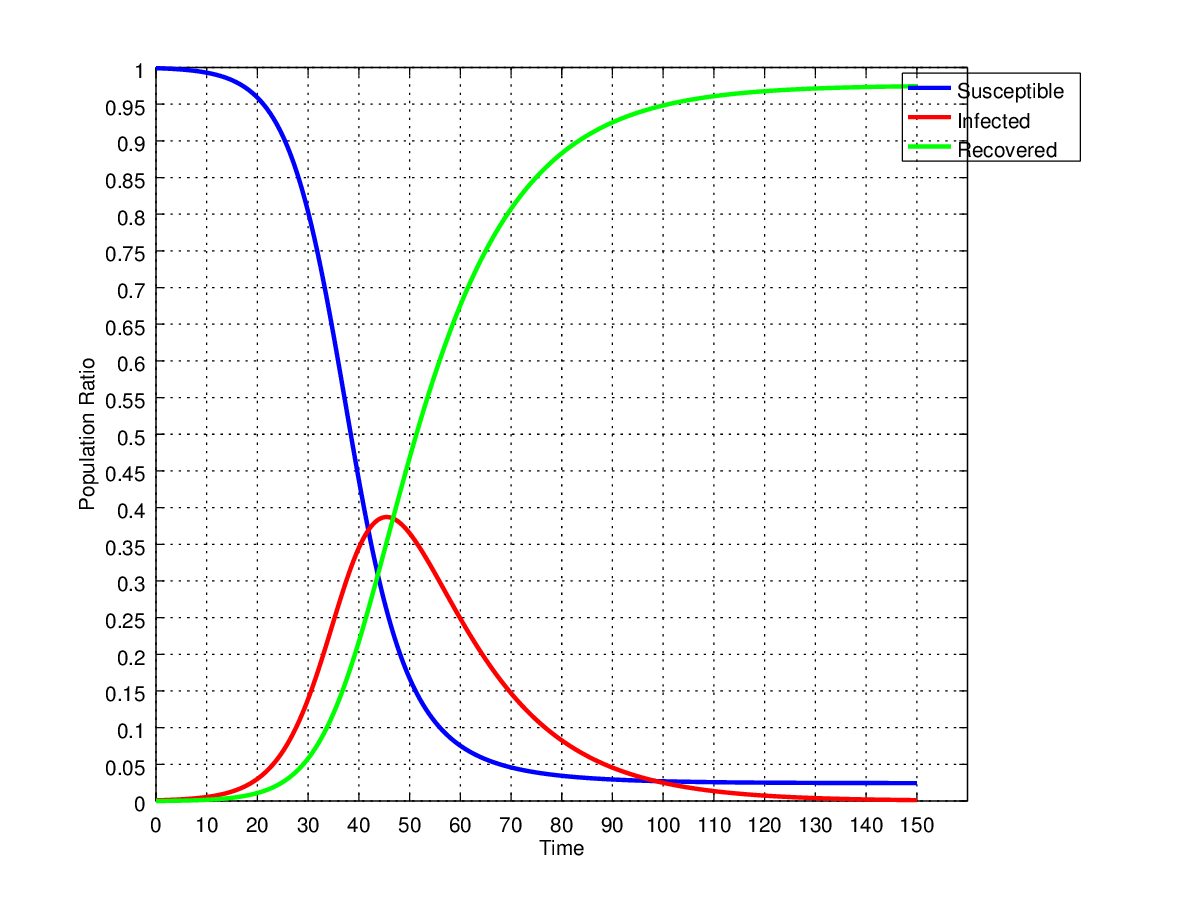
\includegraphics[width=.8\textwidth, angle=0]{./../shared/fig/frsd/SIR_SD_1000agents_150t_01dt.png}
			\caption{$t\Delta = 0.1$}
			\label{fig:sd_plot_0.1dt}
		\end{subfigure}
	\end{tabular}
	
	\caption{Simulating the SIR model with our system dynamics emulation using different time-deltas. Note that although $t\Delta = 0.1$ might seem very close the system dynamic solution, there are still subtle differences to the initial Figure \ref{fig:sir_sd_dynamics} which uses $t\Delta = 0.01$.}
	\label{fig:sd_plots}
\end{center}
\end{figure*}

\subsection{Spatiality and Networks}
When trying to emulate the dynamics of the SIR model using an agent-based approach the question arises what we ultimately gain from doing so when we could have generated the dynamics much quicker and smoother using the system-approach. The difference is that the agent-based approach is a stochastic one and can thus also generate "degenerated" dynamics e.g. in which the disease dies out after a few steps or even can't spread from patient zero - in this case ABS is clearly a benefit as it allows to investigate \textit{alternative futures}, something not possible with system-dynamics in which the disease will never die out prematurely. \\
Another advantage of ABS over the system-dynamics approach is that agents can be heterogeneous and make use of spatial- and/or network-information defining the neighbourhood. We can thus simulate the spread of the disease throughout a population which is laid out on a 2d-grid or one can investigate spreading of the disease throughout a network of agents where some are vaccinated and others not. We provide already suitable environments to simulate these cases and show an example of spreading the disease on a 2d-grid in Figure \ref{fig:sir_spatial}.  

\begin{figure*}
\begin{center}
	\begin{tabular}{c c}
		\begin{subfigure}[b]{0.4\textwidth}
			\centering
			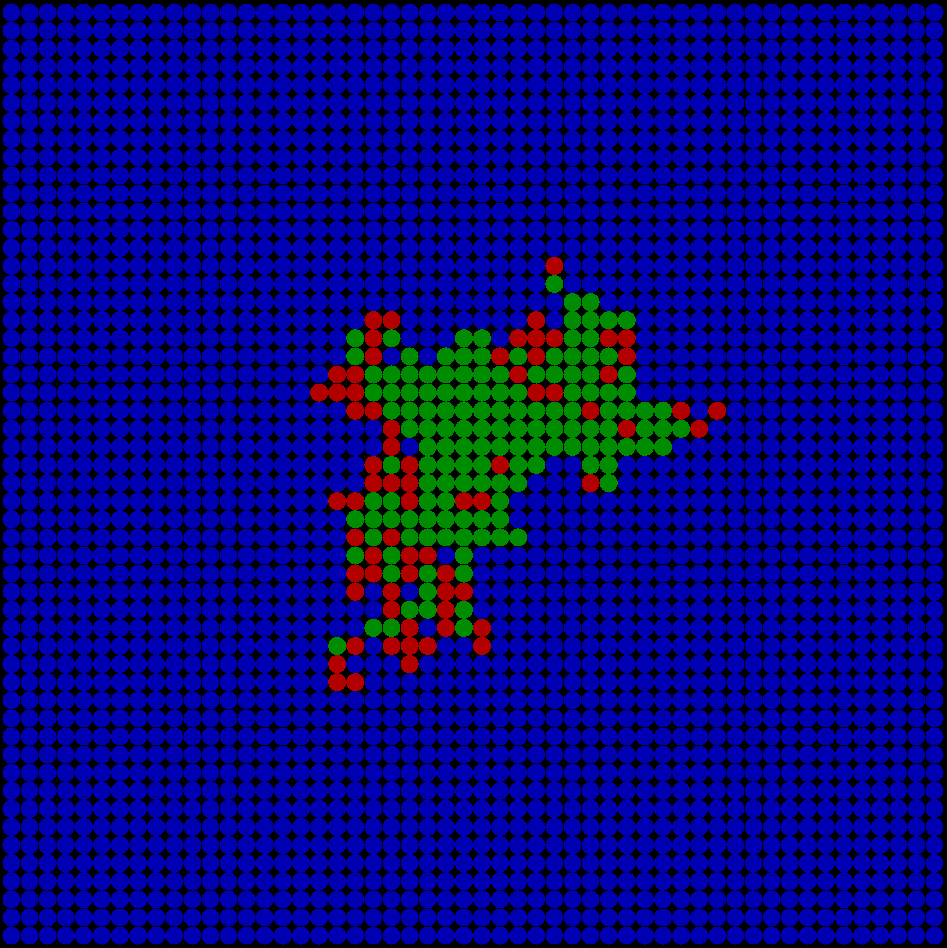
\includegraphics[width=.6\textwidth, angle=0]{./../shared/fig/spatial/SIR_spatial_52x52_92time.png}
			\caption{$t = 92$}
			\label{fig:sir_spatial_92}
		\end{subfigure}

		& 

		\begin{subfigure}[b]{0.4\textwidth}
			\centering
			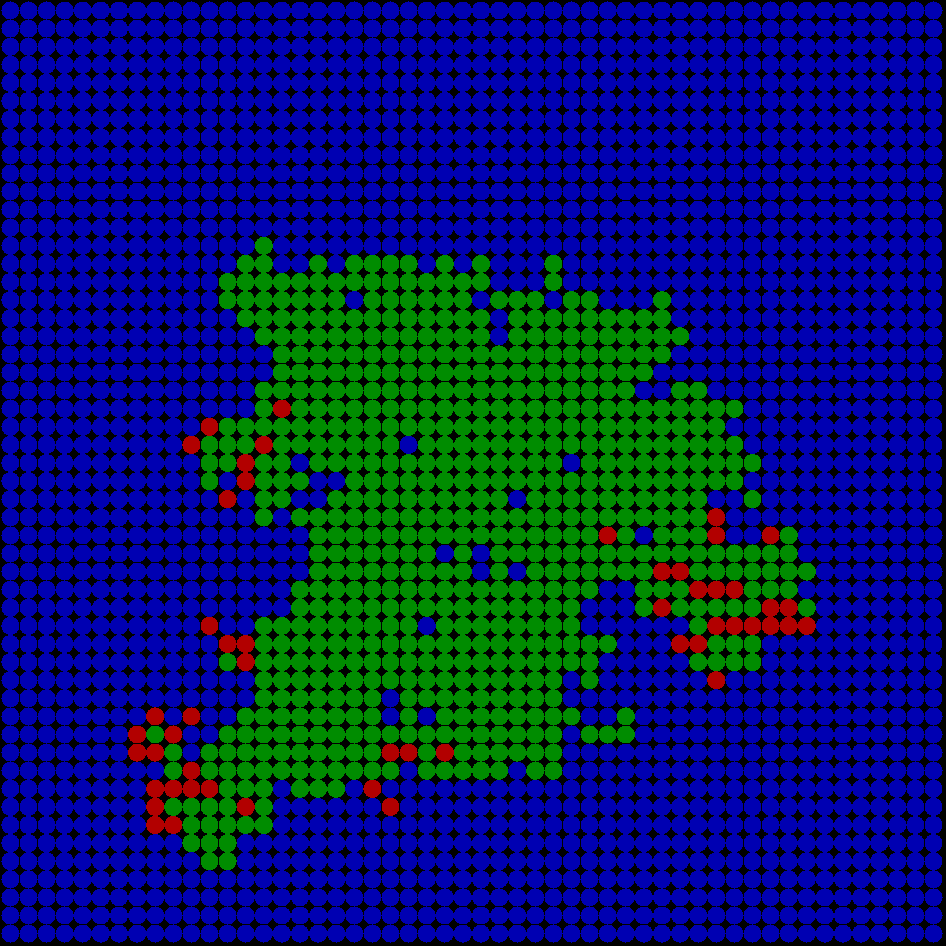
\includegraphics[width=.6\textwidth, angle=0]{./../shared/fig/spatial/SIR_spatial_52x52_200time.png}
			\caption{$t = 200$}
			\label{fig:sir_spatial_200}
		\end{subfigure}

		\\
		
		\begin{subfigure}[b]{0.4\textwidth}
			\centering
			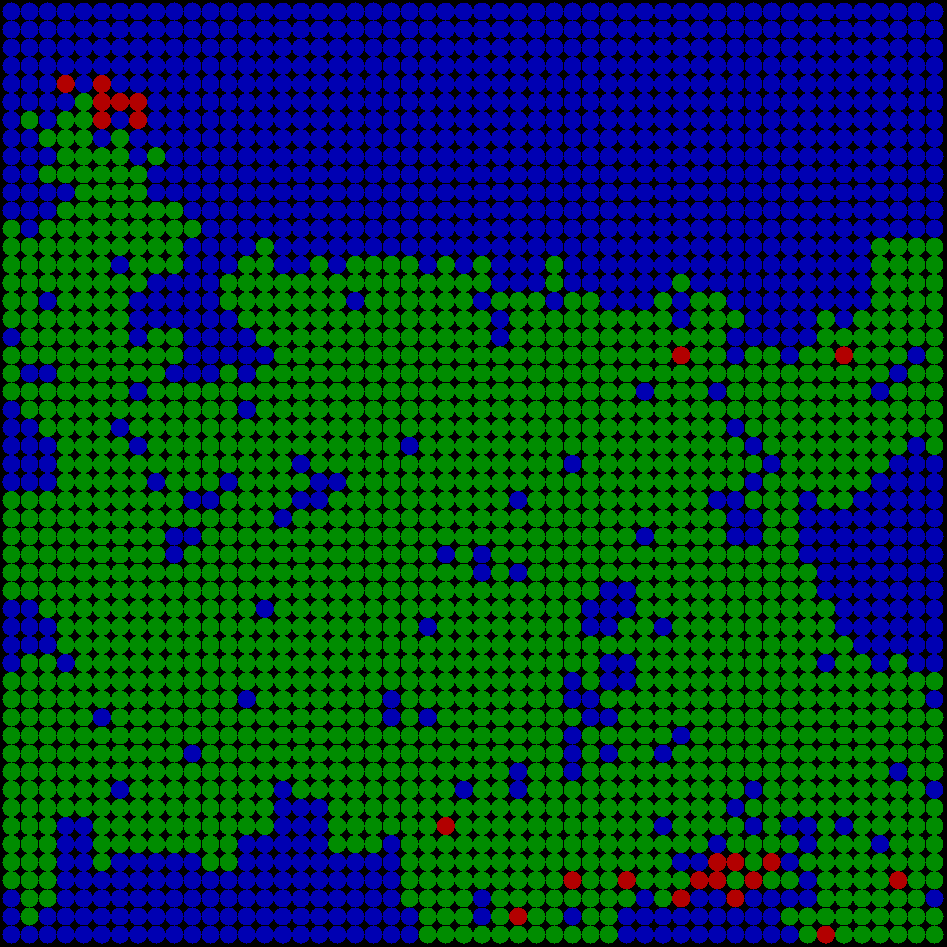
\includegraphics[width=.6\textwidth, angle=0]{./../shared/fig/spatial/SIR_spatial_52x52_440time.png}
			\caption{$t = 440$}
			\label{fig:sir_spatial_440}
		\end{subfigure}
		
		& 
		
		\begin{subfigure}[b]{0.4\textwidth}
			\centering
			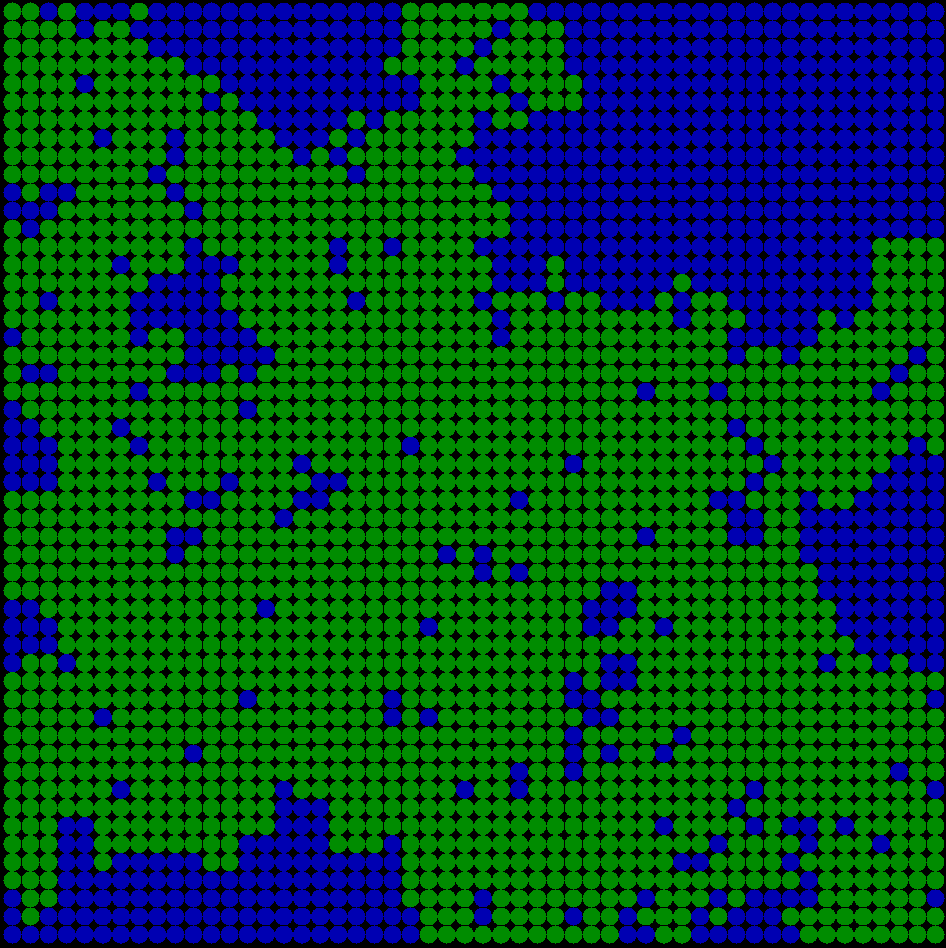
\includegraphics[width=.6\textwidth, angle=0]{./../shared/fig/spatial/SIR_spatial_52x52_873time.png}
			\caption{$t = 873$}
			\label{fig:sir_spatial_873}
		\end{subfigure}
	\end{tabular}
	
	\caption{Simulating SIR on a 52x52 grid with Moore neighbourhood using $t\Delta = 1$. Blue are susceptible, red are infected, green are recovered. The green areas act as protection as infected cannot cross the recovered border: this is particularly visible in the lower right corner of \ref{fig:sir_spatial_440} where the disease has been contained in the blue island and has no means to escape. It may seem that the few remaining infected agents in the top left corner of \ref{fig:sir_spatial_440} will die out soon but still it needs more than the already running simulation-time until the disease actually dies out with the last patient recovering at center top of \ref{fig:sir_spatial_873} at $t = 873$.} 
	\label{fig:sir_spatial}
\end{center}
\end{figure*}

When using a 2d-grid or network one needs to set them up in the initialization code so there is a little more work to do there but the implementation of the agents differ just in one single line, which is where the neighbourhood is picked TODO: refer to appendix code. Instead of \textit{randomAgentIdMsgSource} one uses either \textit{randomNeighbourNodeMsgSource} in the case of a network or \textit{randomNeighbourCellMsgSource} in case of a 2d-grid.

\subsection{Agents as Signals}
Due to the underlying nature and motivation of Functional Reactive Programming and Yampa, agents can be seen as signals which are generated and consumed by a Signal-Function which is the behaviour of an agent.  If an agent does not change the output-signal is constant, if the agent changes e.g. by sending a message, changing its state,... it changes and a dead agent has no signal at all.
The question is if the agents of our agent-based SIR implementation are true signals: do the dynamics change when we sample the system with $t\Delta = 0$? We hypothesize that our agents are true signals, thus they should not change when time does not change because they are completely time-dependent and rely completely on time-semantics. When actually running the simulation with $t\Delta = 0$ one gets the results as in \ref{fig:sir_abs_zero_dt}.

\begin{figure*}
\begin{center}
	\begin{tabular}{c c}
		\begin{subfigure}[b]{0.5\textwidth}
			\centering
			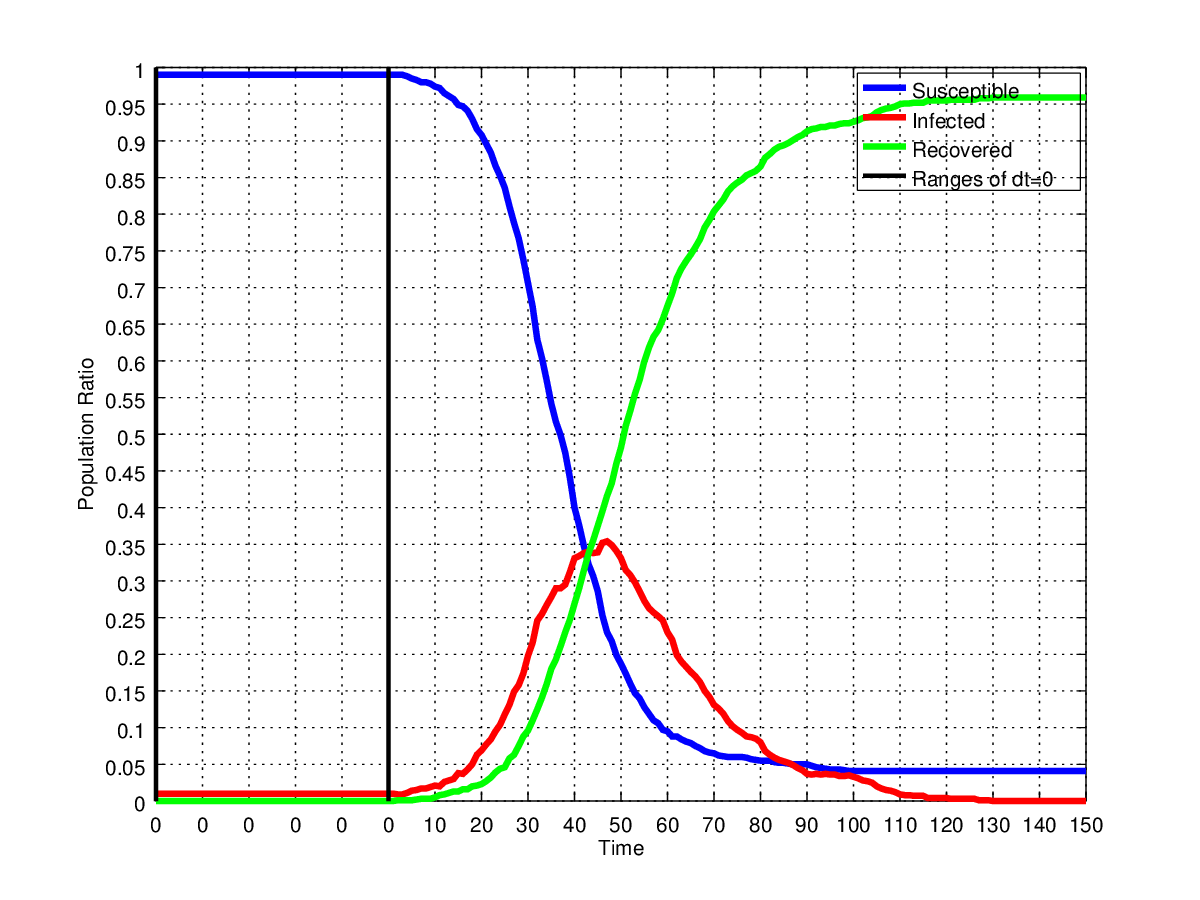
\includegraphics[width=.8\textwidth, angle=0]{./../shared/fig/dtzero/SIR_ABS_zeroDt_start.png}
			\caption{$t\Delta = 0$ from step 0 to 50.}
			\label{fig:sd_plot_10dt}
		\end{subfigure}
	
		& 
		
		\begin{subfigure}[b]{0.5\textwidth}
			\centering
			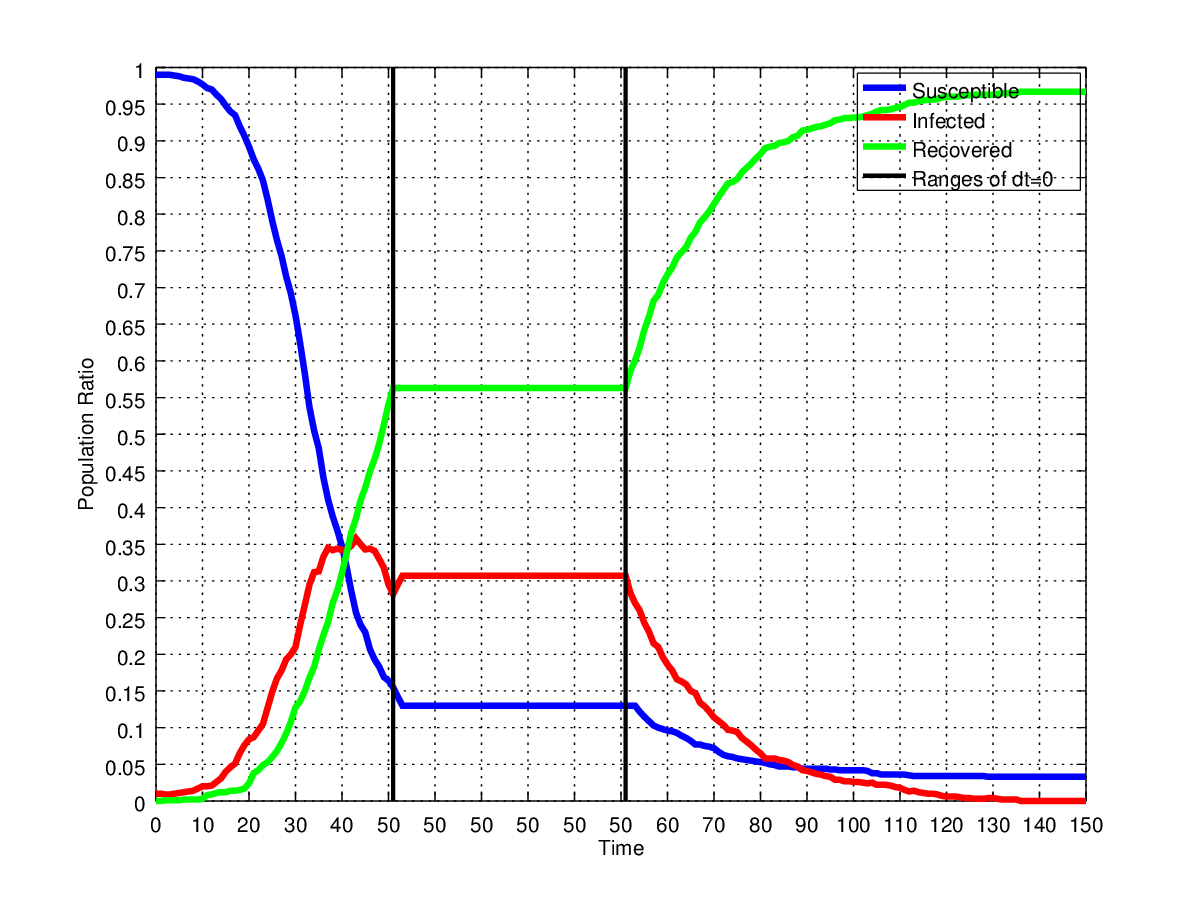
\includegraphics[width=.8\textwidth, angle=0]{./../shared/fig/dtzero/SIR_ABS_zeroDt_mid.png}
			\caption{$t\Delta = 0$ from step 51 to 101.}
			\label{fig:sd_plot_0.01dt}
		\end{subfigure}
	\end{tabular}
	
	\caption{Dynamics of agent-based SIR implementation of 1000 agents running with $t\Delta = 1$ with ranges of $t\Delta = 0$ marked with two vertical black lines.}
	\label{fig:sir_abs_zero_dt}
\end{center}
\end{figure*}

As can be seen  the dynamics are becoming constant \textit{but} with a minor delay: infected increases a bit while susceptible decreases as can be seen in Figure \ref{fig:sir_abs_zero_dt_zoom}. This is due to the delay of message delivery which takes one $t\Delta$, independent of its value - messages are also delivered when $t\Delta = 0$. Only message-generating functions which depend on non-zero $t\Delta$ to generate messages will then stop generate messages. Reactive functions which act on incoming messages can still create change as they do not rely on time-semantics but just on the discrete event of a message-arrival - which is the case in the transition from susceptible to infected.

\begin{figure}
	\centering
	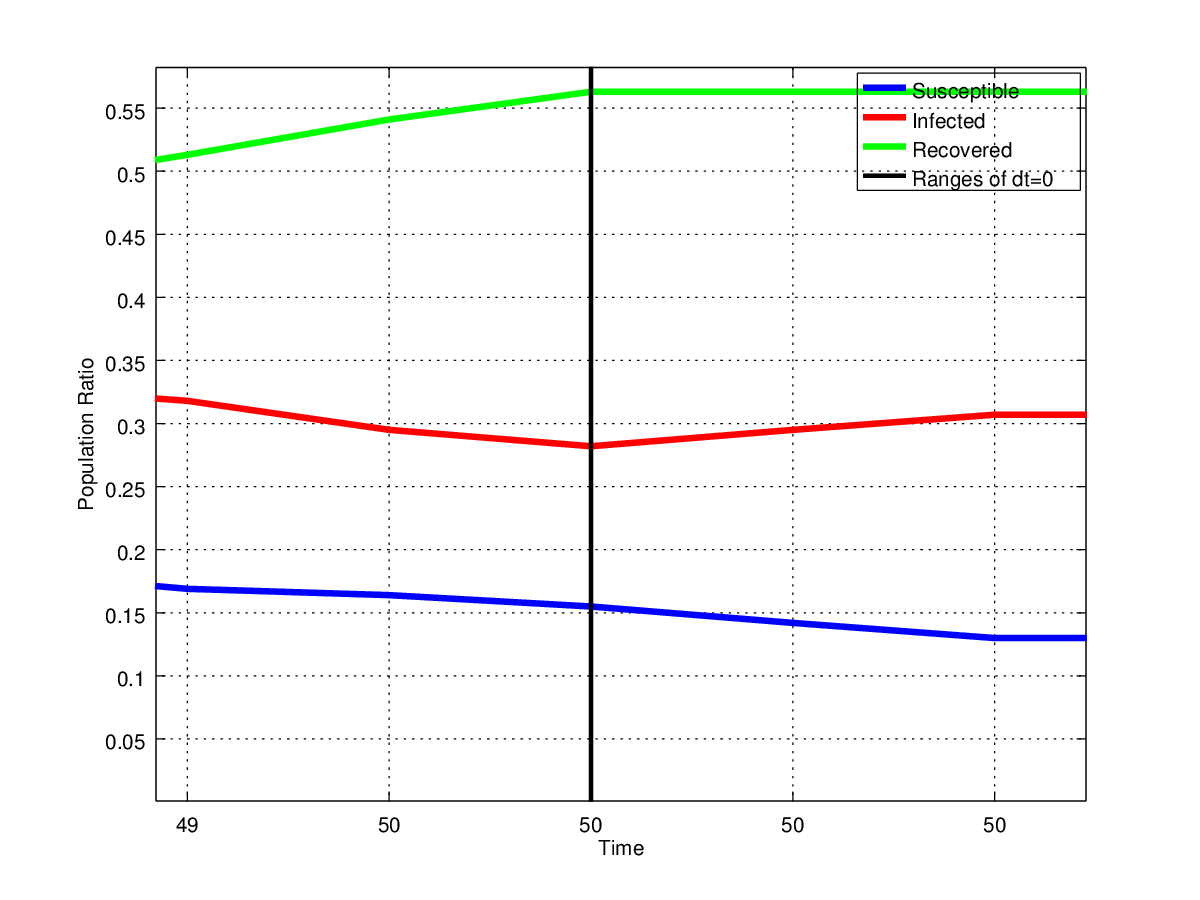
\includegraphics[width=.4\textwidth, angle=0]{./../shared/fig/dtzero/SIR_ABS_zeroDt_mid_zoom.png}
	\caption{Zoom-in to step 51, marked with the black line from where on $t\Delta = 0$ for the next 50 steps. The recovered ratio stays constant but a few agents get infected even \textit{after} having switched to $t\Delta = 0$ which happens due to the message-delivery lag. After all messages have been delivered, the signal stays constant until non-zero $t\Delta$ are turned on again.}
	\label{fig:sir_abs_zero_dt_zoom}
\end{figure}

Note that agents of non-time semantic models won't exhibit this behaviour - the dynamics will change even in case of a $t\Delta = 0$ - they just act on every update and don't care about the time-delta and just assume that every update occurs after a $t\Delta$ independent of the actual value of it. We implemented the function \textit{doRepeatedlyEvery} which allows to transform a non-time semantic agent-behaviour into one. It is built on Yampas \textit{repeatedly} function and has the following signature:

\begin{minted}[fontsize=\footnotesize]{haskell}
doRepeatedlyEvery :: Time -> AgentBehaviour s m e -> AgentBehaviour s m e
\end{minted}

This function takes a time interval and an agent-behaviour signal-function and returns a new agent-behaviour signal-function which runs the argument signal-function every time-interval. Note that this function is subject to sampling-issues too e.g. when the time-interval is very small one needs to run the simulation with a $t\Delta \leq Time$ otherwise the dynamics would show delayed activation of the agent-behaviour.

\subsection{Randomness}
It is important to note that if we disable super-sampling and run the simulation for a given time \textit{t} but with e.g. two different $t\Delta$ we would end up with two different results, even if the $t\Delta$ are small enough to sample the time-dependent functions sufficiently. Also if we use super-sampling with $t\Delta = 1.0$ and create the exact same number of samples as when using no super-sampling but smaller $t\Delta$, then we also end up with different results.
The reason for this behaviour is that all these time-dependent functions ultimately build upon drawing from random-distributions. With different $t\Delta$ we are generating random-samples to a greater or lesser extent, which would result in different random-number sequences which in turn ultimately leads to slightly different dynamics. When generating a plot of the dynamics this is not as visible, also this is the reason why one generates multiple replications, but this behaviour becomes strikingly apparent when simulating the SIR model on a 2d-grid as can be seen in Figure \ref{fig:sir_abs_timeDeltas_reproduce}.

\begin{figure*}
\begin{center}
	\begin{tabular}{c c}
		\begin{subfigure}[b]{0.4\textwidth}
			\centering
			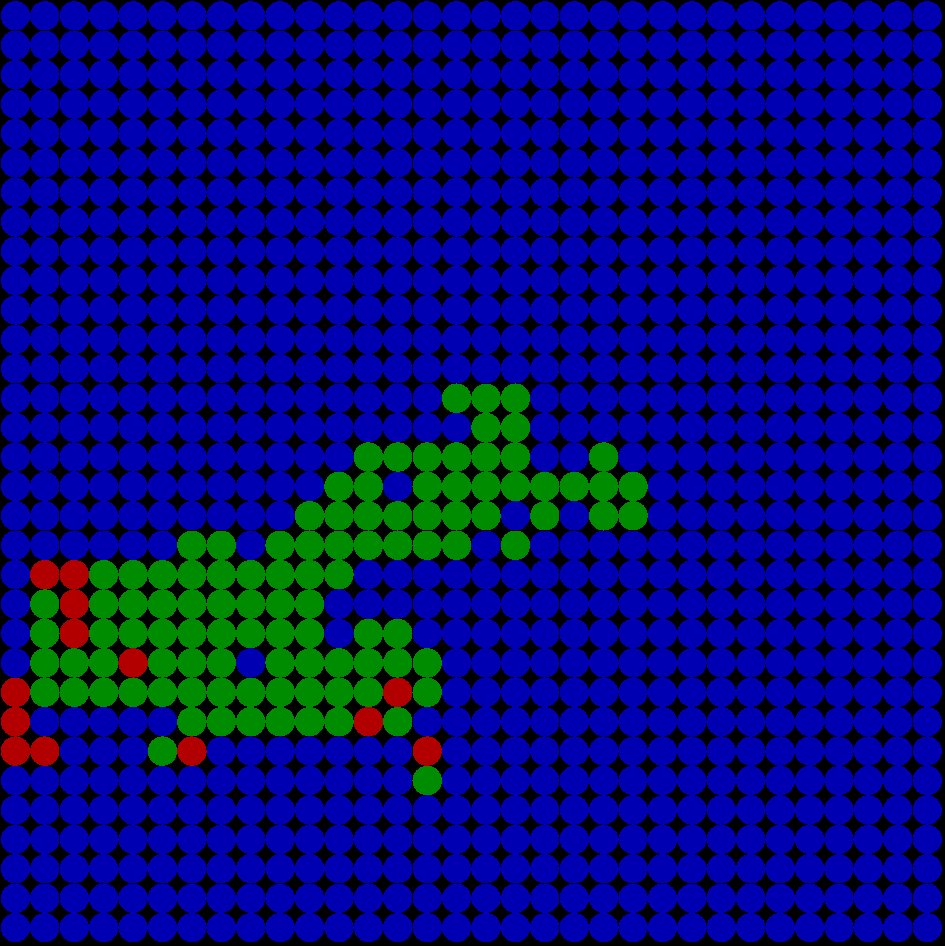
\includegraphics[width=.7\textwidth, angle=0]{./../shared/fig/randomness/SIR_32x32_200time_01delta_noSS.png}
			\caption{$t\Delta = 0.1$, no super-sampling}
			\label{fig:sir_abs_timeDeltas_randomness_dt01}
		\end{subfigure}
	
		& 
		
		\begin{subfigure}[b]{0.4\textwidth}
			\centering
			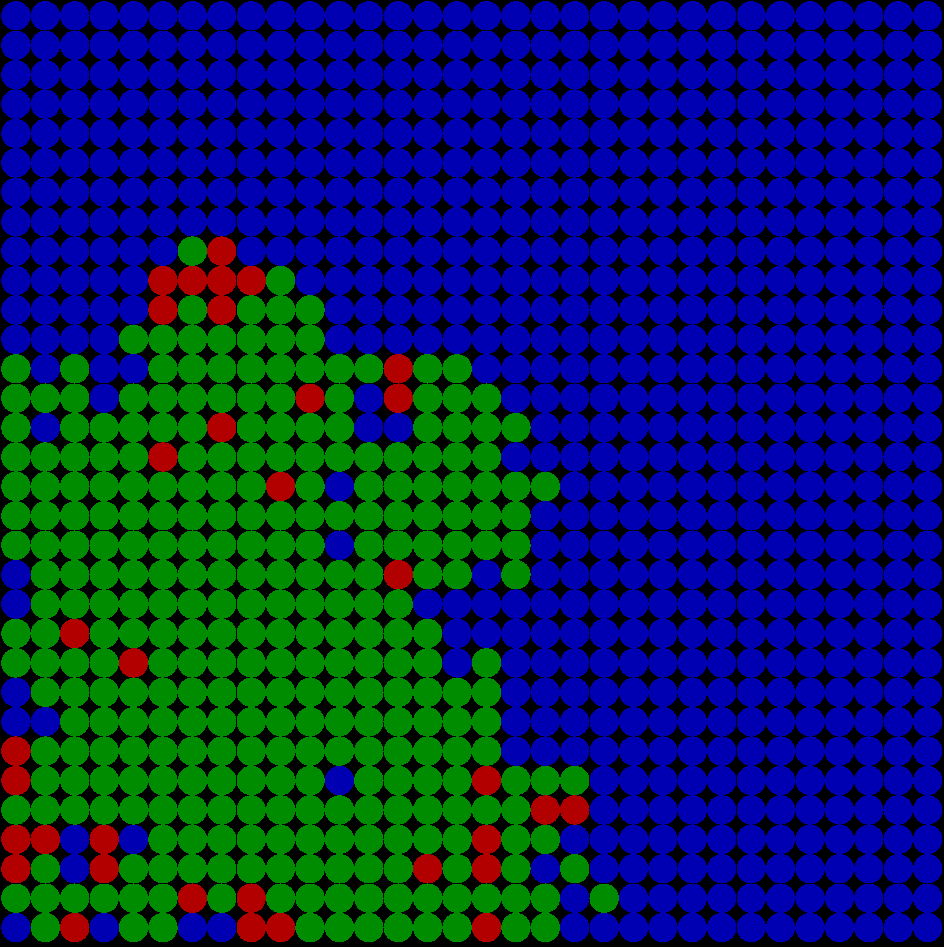
\includegraphics[width=.7\textwidth, angle=0]{./../shared/fig/randomness/SIR_32x32_200time_001delta_noSS.png}
			\caption{$t\Delta = 0.01$, no super-sampling}
			\label{fig:sir_abs_timeDeltas_randomness_dt001}
		\end{subfigure}
		
		\\

		\begin{subfigure}[b]{0.4\textwidth}
			\centering
			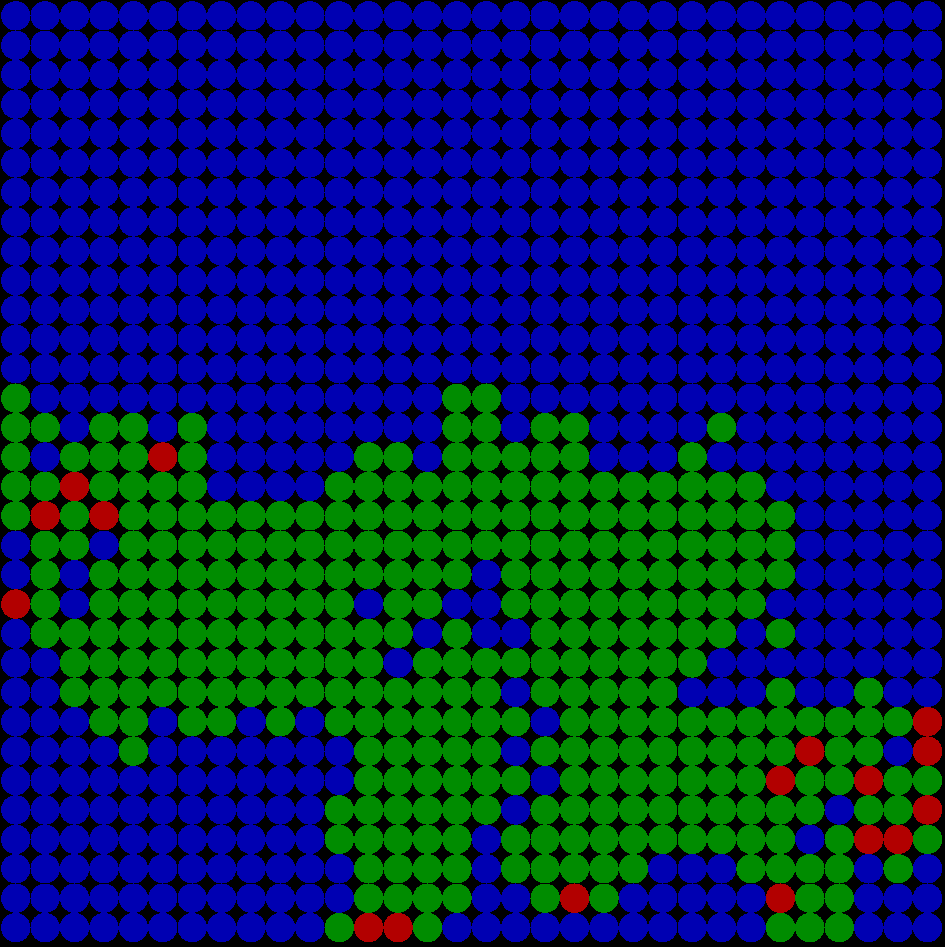
\includegraphics[width=.7\textwidth, angle=0]{./../shared/fig/randomness/SIR_32x32_200time_10delta_ss10.png}
			\caption{$t\Delta = 1.0$ with 10 super-samples}
			\label{fig:sir_abs_timeDeltas_randomness_dt10_ss10}
		\end{subfigure}
		
		&
		
		\begin{subfigure}[b]{0.4\textwidth}
			\centering
			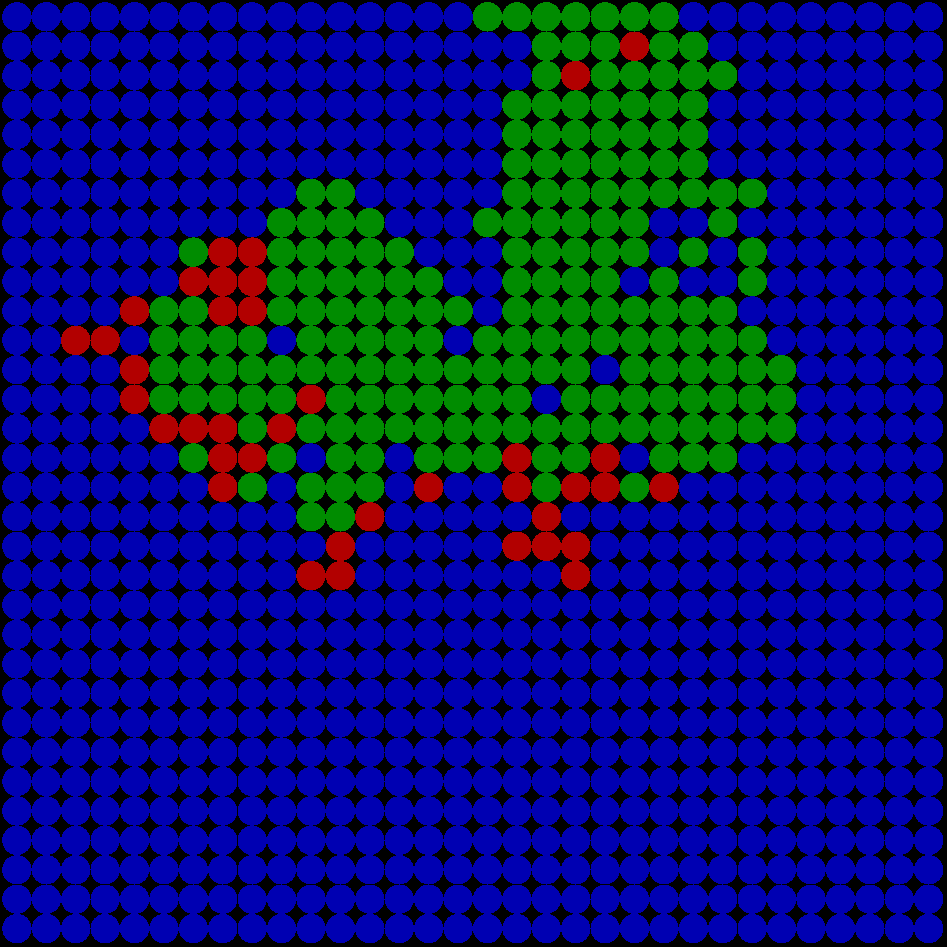
\includegraphics[width=.7\textwidth, angle=0]{./../shared/fig/randomness/SIR_32x32_200time_10delta_ss100.png}
			\caption{$t\Delta = 1.0$ with 100 super-samples}
			\label{fig:sir_abs_timeDeltas_randomness_dt10_ss100}
		\end{subfigure}
	\end{tabular}
	
	\caption{Comparing results on 32x32 grid after $t = 200$ but with different $t\Delta$ and different number of super-samples. Note that a $t\Delta = 0.1$ is clearly not enough, whereas the others result in much more recovered agents.}
	\label{fig:sir_abs_timeDeltas_randomness}
\end{center}
\end{figure*}

\subsection{Message Round-trip Time}
When reflecting on the messaging mechanism it becomes apparent that a round-trip from sender to receiver and back takes $2 t\Delta$. A round-trip happens in our agent-based SIR approach to implement the transition from infected to susceptible - susceptible agents send Contact Susceptible messages to random agents (except itself) where only infected agents reply with a Contact Infected message. This means that it takes $2 t\Delta$ until a susceptible agent might get infected. This becomes an issue if we want to match the dynamics of our agent-based approach to the system-dynamics one in which no time-delay happens - the agents act instantaneous with each other during one time-step. 
We have two solutions for this problem: either we resort to \textit{conversations} or we increase the global sampling frequency of the system which matches the \textit{message frequency} of messages which are subject to round-trips. Implementing conversations is only available in the \textit{sequential} update-strategy and is much more cumbersome, so we followed the approach of increasing the frequency. We tried different frequencies and found that $t\Delta = 0.1$ results in a sufficiently good approximation to the system dynamics solution as can be seen in Figure TODO.

\subsection{Recursive ABS}
Due to the inherent recursive nature of functional programming we came up with the idea of \textit{recursive} ABS in which agents can recursively run the simulation within the simulation which would allow them to project their own actions into the future. So far it only exists as a proof-of-concept and we are currently only aware of a single model \cite{gilmer_recursive_2000} in the field of ABS which does recursive simulation. The implementation of recursive ABS is very natural due to the explicit data-flow and lack of side-effects which eases the task very much. Unfortunately we cannot go into detail of our approach as it is beyond the scope of the paper.

\subsection{Advantages}
We now look at a number of advantages this functional reactive approach to ABS has over to the traditional imperative, object-oriented implementation approaches done in Phyton, Java, C++.

\subsubsection{Code close to specification}
As becomes directly evident when looking at the code of the agent-based implementation in Appendix \ref{app:abs_code} and system dynamics implementation in Appendix \ref{app:sd_code}, it looks very much like a specification. By creating this EDSL which allows to express powerful time-semantics it is possible to now create an ABS in a declarative style in Haskell where agent-implementation looks like a model-specification thus being correct by definition.
arrowized programming is optional and only required when utilizing yampas time-semantics. if the model does not rely on time-semantics, it can use monadic-programming by building on the existing monadic functions in the EDSL which allow to run in the State-Monad which simplifies things very much
	- when to use yampas arrowized programing: time-semantics, simple state-chart agents 
	- when not using yampas facilities: in all the other cases e.g. SugarScape is such a case as it proceeds in unit time-steps and all agents act in every time-step
	
\subsubsection{Being pure}
Because no part of the simulation runs in the IO monad \footnote{Except when using graphical rendering, but then only the rendering happens in the IO Monad - the simulation step is always a pure computation} and we do not use unsafePerformIO \footnote{We actually do use it for generating unique agent-ids for newly created agents. This is necessary because need to guarantee that two invocations will result in two different ids, which would be difficult / impossible when running the simulation in the \textit{parallel} update-strategy. This is not a problem as long as an agent does not rely on the absolute value of an agent-id but just uses it as an opaque identifier for sending/receiving.} we can rule out a serious class of bugs caused by implicit data-dependencies and side-effects which can occur in traditional imperative implementations.
Also we can statically guarantee the reproducibility of the simulation because of that. There are no side effects possible within the agents which would result in differences between same runs (e.g. file access, networking, threading). Every agent has access to its own random-number generator, allowing randomness to occur in the simulation but the random-generator seed is fixed in the beginning and can never be changed within an agent to come from e.g. the current system time, which would require to run within the IO Monad. This means that after initialising the agents, which \textit{could} run in the IO Monad, the simulation itself runs completely deterministic.
We provide functionality to render the output to a window (using the library Gloss) or writing to a text-file, meaning, parts of the simulation would run in the IO Monad. Here we rely on Yampas \textit{reactimate} function which provides a well-defined way of communicating with the world in such a system. This function provides the $t\Delta$ for the next step, which \textit{could} come from IO Monad but we keep the $t\Delta$ always fixed, thus removing another source of non-reproducibility where e.g. $t\Delta$ is influenced by sytem-dependent non-deterministic rendering-performance every step as happens in games or described by \cite{perez_testing_2017} in the context of FRP.

\subsubsection{Robust time handling}
cant mess around with time because delta-time is hidden from you (intentional design-decision by Yampa). this would be only very difficult and cumbersome to achieve in an object-oriented approach. TODO: experiment with it in Java - how could we actually implement this? I think it is impossible: may only achieve this through complicated application of patterns and inheritance but then has the problem of how to update the dt and more important how to deal with functions like integral which accumulates a value through closures and continuations. We could do this in OO by having a general base-class e.g. ContinuousTime which provides functions like updateDt and integrate, but we could only accumulate a single integral value.
TODO: this is also the case in e.g. RePast simphony in which one never deals with time-deltas but interacts with the scheduler through anotations

\subsubsection{Replications}
get replications for free without having to worry about side-effects and can even run them in parallel without headaches. TODO: need a little bit of discussion here as it is not that easy: we need to swap random-number generators out for new one in every replication, both in agents and environments

\subsection{Disadvantages}
We identify two main disadvantages.

\subsubsection{Performance}
Performance is currently no where near imperative object-oriented implementations. The reason for this is that we don't have in-place updates of data-structures and make no use of references. This results in lots of copying which is simply not necessary in the imperative languages with implicit effects. Also it is much more difficult to reason about time and space in our approach. Thus we see performance clearly as the main drawback of the functional approach and the only real advantage of the imperative approach over our.

\subsubsection{Steep learning curve}
Our approach is quite advanced in three ways. First it builds on the already quite involved FRP paradigm. Second it forces one to think properly of time-semantics of the model, how to sample it, how small $t \Delta$ should be and whether one needs super-sampling or not and if yes how many samples one should take. Third it requires to think about agent-interaction and update-strategies, whether one should use conversations which forces one to run sequentially or if one can run agents in parallel and use normal messaging which but incurs a time-delay which in turn would need to be considered when setting the $t \Delta$.